\documentclass[10pt, a4paper]{article}
%Gummi|065|=)
\usepackage{graphicx}
\usepackage{CJK}
\usepackage{amsmath}
\usepackage{algorithm}
\usepackage[noend]{algpseudocode}
\begin{CJK}{UTF8}{gbsn}


\title{\textbf{Alogrithm exercise }}


\author{ywjia@mail.ustc.edu.cn\\
		SA14011066\\
		贾亚伟}
\date{2014-10-23}

\begin{document}

\maketitle
\DeclareGraphicsExtensions{.pdf,.png,.jpg}


\section{ex1}
ex1.c in ex director \\

\textbf{result as follows:}
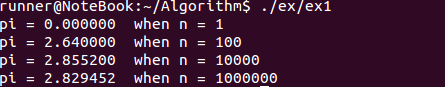
\includegraphics{./ex1pic}
\section{ex2}
ex2.c in ex director 



\section{ex3}
ex3.c in ex director


\section{ex4}
\textbf{Question:} \\
Assume $\epsilon, \delta$ is constant within $(0, 1)$, prove: \\
If I is the correct value of $\int_0^1{f(x)dx}$, and h is the return value of alogrithm "HitorMiss", Then $Prob[|h-I| < \epsilon] \geq 1 - \delta$ when $n \geq I(1-I)/\epsilon^{2}\delta$. \\
 \textbf{Prove:}\\
Assume we hit the area n times and there are  k points scatterd under the area $f(x)$.Apparently, the random X that the number of points scattered under $f(x)$ is Binomial Distribution, that is $P_r(X = k) = C_n^{k}p^{k}(1-p)^{n-k}$
then, $E(X) = np, Var(X) = np(1-p)$.\\
the h that HitOrMiss return is $k/n$, So $h = X/n, E(h) = E(X/n) = p = k/n = I, Var(h) = Var(X/n) = \frac{p(1-p)}{n} = \delta^{2}$. \\
According to Chebyshev's inequality $Pr(|h - I| \leq \epsilon) \geq 1 - \delta^{2}/\epsilon^{2} $  And according to the cond: $n \geq I(1-I)/\epsilon^{2}\delta$, So we have $Pr(|h - I| \leq \epsilon )\geq 1 - \frac{p(1-p)}{\epsilon^{2}n} \geq 1 - \frac{p(1-p)}{\epsilon^{2}}\frac{\epsilon^{2}\delta}{I(1-I)} = 1 - \delta.\\
Q.E.D$

\section{ex5}

ex5.py in ex director

\section{ex6}

\textbf{问题:}
写一Sherwood算法C 与算法A,B,D比较,并给出实验结果。

\textbf{答案:} \\
程序ex6.c 及结果 见 ex 文件夹。 

\section{ex7}

\textbf{问题:} 
证明当放置第k+1个皇后时, 若有多个位置是开放的, 则算法QueensLV选中其中一位置的概率相等。


证: 假设在放置k+1个皇后时,有nb个位置可以放置, 并假设选中了第i个位置, 则其概率$p(i) = \frac{1}{i}\times\frac{i}{i+11}\times \cdots \times \frac{nb-1}{nb} = \frac{1}{nb}$ 即选中其中一个位置的概率均相等, 为$\frac{1}{nb}$。 

\section{ex8}

写一算法,求n=12-20时最优的StepVegas值。
\begin{algorithm}
\caption{求StepVegas最优值}\label{euclid}
\begin{algorithmic}[1]
\Procedure{OptimalStepVegas}{}
\State $\textit{mintime} \gets \infty$
\State $\textit{k} \gets 0$

\For{from $n = 12$ to  20 }
	\For{from $\textit{k} = 0$ to 20}
	\State $\textit{time} \gets QueensLv(n, success, \textit{k})$
	\If{$\textit{time} < \textit{mintime}$}
		\State $\textit{mintime} \gets \textit{time}$
		\State $\textit{stepVegas} \gets k$
 	\EndIf
 	\EndFor
 	
 	\State Print $The Count of Queens:n,  Optimal StepVegas Value is : stepVegas$
\EndFor

\EndProcedure
\end{algorithmic}
\end{algorithm}

% 分布式算法部分习题
\section{ex2.1}
\textbf{问题:}分析在同步和异步模型下,convergecast 算法的时间复杂性。





\end{CJK}
\end{document}

